\documentclass[12pt,letterpaper]{article}
\usepackage{graphicx,textcomp}
\usepackage{natbib}
\usepackage{setspace}
\usepackage{fullpage}
\usepackage{color}
\usepackage[reqno]{amsmath}
\usepackage{amsthm}
\usepackage{fancyvrb}
\usepackage{amssymb,enumerate}
\usepackage[all]{xy}
\usepackage{endnotes}
\usepackage{lscape}
\newtheorem{com}{Comment}
\usepackage{float}
\usepackage{hyperref}
\newtheorem{lem} {Lemma}
\newtheorem{prop}{Proposition}
\newtheorem{thm}{Theorem}
\newtheorem{defn}{Definition}
\newtheorem{cor}{Corollary}
\newtheorem{obs}{Observation}
\usepackage[compact]{titlesec}
\usepackage{dcolumn}
\usepackage{tikz}
\usetikzlibrary{arrows}
\usepackage{multirow}
\usepackage{xcolor}
\newcolumntype{.}{D{.}{.}{-1}}
\newcolumntype{d}[1]{D{.}{.}{#1}}
\definecolor{light-gray}{gray}{0.65}
\usepackage{url}
\usepackage{listings}
\usepackage{color}
\usepackage{pdfpages}  


\definecolor{codegreen}{rgb}{0,0.6,0}
\definecolor{codegray}{rgb}{0.5,0.5,0.5}
\definecolor{codepurple}{rgb}{0.58,0,0.82}
\definecolor{backcolour}{rgb}{0.95,0.95,0.92}

\lstdefinestyle{mystyle}{
	backgroundcolor=\color{backcolour},   
	commentstyle=\color{codegreen},
	keywordstyle=\color{magenta},
	numberstyle=\tiny\color{codegray},
	stringstyle=\color{codepurple},
	basicstyle=\footnotesize,
	breakatwhitespace=false,         
	breaklines=true,                 
	captionpos=b,                    
	keepspaces=true,                 
	numbers=left,                    
	numbersep=5pt,                  
	showspaces=false,                
	showstringspaces=false,
	showtabs=false,                  
	tabsize=2
}
\lstset{style=mystyle}
\newcommand{\Sref}[1]{Section~\ref{#1}}
\newtheorem{hyp}{Hypothesis}

\title{Problem Set 1}
\date{Due: January 28, 2026}
\author{Data Visualisation for Social Scientists}

\begin{document}
	\maketitle
	
	\section*{Instructions}
	\begin{itemize}
	\item Please show your work! You may lose points by simply writing in the answer. If the problem requires you to execute commands in \texttt{R}, please include the code you used to get your answers. Please also include the \texttt{.R} file that contains your code. If you are not sure if work needs to be shown for a particular problem, please ask.
\item Your homework should be submitted electronically on GitHub.
\item This problem set is due before 23:59 on Wednesday January 28, 2026. No late assignments will be accepted.
	\end{itemize}
	
	\vspace{1cm}
	\section*{Roll Call Votes in the European Parliament}

\subsection*{Data Manipulation}
First, you need to \href{https://personal.lse.ac.uk/hix/HixNouryRolandEPdata.HTM}{download data} from the first six elected European Parliaments on each MEP and how they voted in each recorded roll-call vote.

\vspace{.25cm}

\begin{enumerate}
\item Load these datasets into your global environment:
\begin{itemize}
	\item \texttt{mep\_info\_26Jul11.xls} (MEP characteristics, EP1–EP5)
	\item \texttt{rcv\_ep1.txt} (EP1 roll-call votes)
\end{itemize}

	\lstinputlisting[firstline=1,lastline=12]{PS01_RS.r}

\item Briefly describe (2–3 sentences each) the unit of analysis and key variables in each of these two datasets.

\begin{enumerate}
	\item \textbf{mep\_info\_26Jul11.xls (MEP characteristics)}\\
	\textit{Unit of analysis:} Each row represents an individual Member of the European Parliament (MEP) across the first five European Parliaments (EP1--EP5).\\
	\vspace{.25cm}
	\textit{Key variables:} The dataset includes MEP identifiers (e.g., MEP\_ID), personal characteristics (such as name), political affiliation (national party and European Parliament group), country of representation, and ideological positioning variables. This dataset describes attributes of MEPs rather than their voting behavior.
	
	\item \textbf{rcv\_ep1.txt (EP1 roll-call votes)}\\
	\textit{Unit of analysis:} Each row represents a single vote cast by an individual MEP in a recorded roll-call vote during the first European Parliament (EP1).\\
	\textit{Key variables:} Key variables include the MEP identifier, roll-call vote identifier, and the recorded vote decision (e.g., Yes, No, Abstain, Present but did not vote, or Absent). This dataset captures individual voting behavior on legislative decisions.
\end{enumerate}




\item The \texttt{rcv\_ep1} data are in a wide format, with V1, V2, …, Vn as separate vote columns.
\begin{itemize}
	\item Identify which columns are ID/metadata (\textit{MEPID, MEPNAME, MS, NP, EPG}) and which columns are vote decisions ($V_1$…$V_n$). Tidy the voting data such that each row/observation is a single vote for a single MEP.
	
	\lstinputlisting[firstline=14,lastline=22]{PS01_RS.r}

	\item Create a summary table of counts of decision categories (e.g. Yes/No/Abstain/Present but did not vote/Absent) across all votes.
	
	\vspace{1cm}
	
		\lstinputlisting[firstline=23,lastline=40]{PS01_RS.r}
		\vspace{1cm}
		\begin{table}[ht]
			\centering
			\begin{tabular}{l r}
				\hline
				\textbf{Decision} & \textbf{Count} \\
				\hline
				Absent & 109{,}224 \\
				Present but did not vote & 103{,}618 \\
				Not a member & 99{,}753 \\
				Yes & 88{,}185 \\
				No & 75{,}171 \\
				Abstain & 9{,}577 \\
				\hline
			\end{tabular}
			\caption{Distribution of vote decisions in EP1 roll-call votes}
			\label{tab:vote-decisions}
		\end{table}
		
		
\end{itemize}
\item  Construct a new dataset that combines MEP-level information with their vote decisions from EP1 in long format (from part 3). Check for missingness.
\vspace{1cm}
	\lstinputlisting[firstline=45,lastline=54]{PS01_RS.r}
	\vspace{1cm}
	\begin{table}[ht]
		\centering
		\begin{tabular}{r r r r r r r r}
			\hline
			\textbf{MEPID} & \textbf{MEPNAME} & \textbf{MS} & \textbf{NP} & \textbf{EPG} & \textbf{vote\_id} & \textbf{decision} & \textbf{decision\_label} \\
			\hline
			0 & 0 & 0 & 0 & 0 & 0 & 0 & 0 \\
			\hline
		\end{tabular}
		\caption{Example observation from the combined EP1 voting dataset}
		\label{tab:ep1-example-row}
	\end{table}
	

\item Compute, for each EP group in EP1:
\begin{itemize}
	\item The mean rate of Yes votes (Yes over Yes+No+Abstain) across all roll calls.
	\lstinputlisting[firstline=57,lastline=78]{PS01_RS.r}
	\begin{table}[ht]
		\centering
		\begin{tabular}{l r}
			\hline
			\textbf{EP Group} & \textbf{Mean Yes Rate} \\
			\hline
			N & 0.613 \\
			S & 0.563 \\
			E & 0.532 \\
			G & 0.514 \\
			M & 0.512 \\
			L & 0.495 \\
			R & 0.486 \\
			C & 0.437 \\
			\hline
		\end{tabular}
		\caption{Average proportion of Yes votes by EP group in EP1}
		\label{tab:mean-yes-epg}
	\end{table}
	
	\item The mean abstention rate.
	\vspace{1cm}
	\lstinputlisting[firstline=81,lastline=103]{PS01_RS.r}
	\begin{table}[ht]
		\centering
		\begin{tabular}{l r}
			\hline
			\textbf{EP Group} & \textbf{Mean Abstention Rate} \\
			\hline
			R & 0.2690 \\
			M & 0.0893 \\
			G & 0.0806 \\
			C & 0.0725 \\
			L & 0.0654 \\
			S & 0.0598 \\
			N & 0.0580 \\
			E & 0.0215 \\
			\hline
		\end{tabular}
		\caption{Average proportion of abstentions by EP group in EP1}
		\label{tab:mean-abstain-epg}
	\end{table}
	
	
	\item The mean vote preferences along the two contested dimensions (NOM-D1 and NOM-D2).
	\lstinputlisting[firstline=105,lastline=151]{PS01_RS.r}
	\vspace{10cm}
	\begin{table}[ht]
		\centering
		\begin{tabular}{l r r}
			\hline
			\textbf{EP Group} & \textbf{Mean NOM-D1} & \textbf{Mean NOM-D2} \\
			\hline
			R & -0.586 & -0.0419 \\
			M & -0.357 & -0.2010 \\
			S & -0.0980 & 0.2610 \\
			N & 0.250 & -0.3860 \\
			G & 0.280 & -0.8180 \\
			L & 0.409 & -0.3240 \\
			E & 0.512 & -0.2770 \\
			C & 0.811 & 0.5300 \\
			0 & NaN & NaN \\
			\hline
		\end{tabular}
		\caption{Average NOMINATE coordinates (Dimension 1 and Dimension 2) by EP group in EP1}
		\label{tab:mean-nominate-epg}
	\end{table}
	
\end{itemize}
\end{enumerate}

\subsection*{Data Visualization}

\begin{enumerate}
	\item Plot the distribution of the first NOMINATE dimension by EP group, and explain any trends you see.
	\lstinputlisting[firstline=153,lastline=168]{PS01_RS.r}
	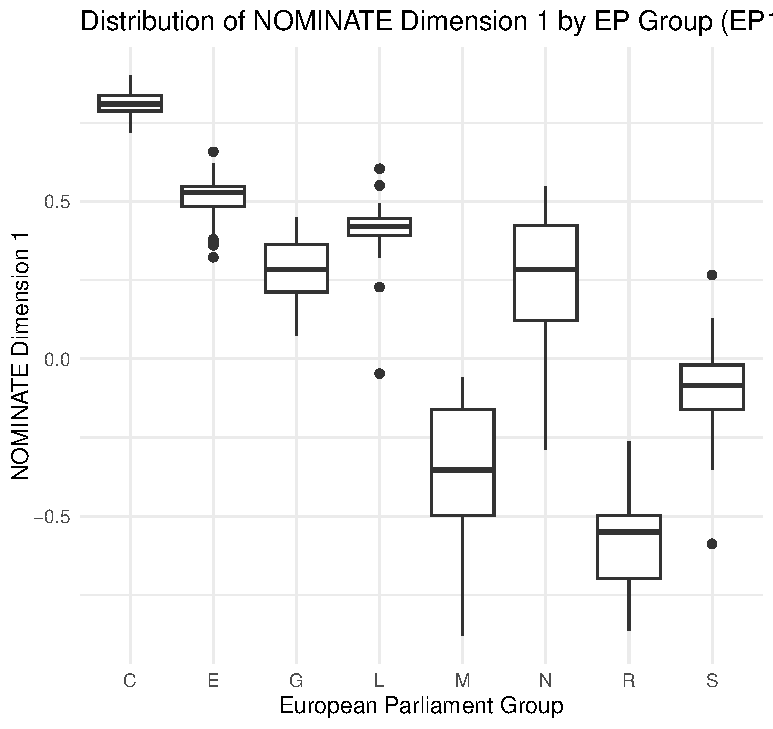
\includepdf[pages=-, scale=0.8]{plot1.pdf}
	\textbf{The plot shows clear differences in NOM-D1 across EP groups, with left-leaning groups concentrated at lower values and right-leaning groups at higher values. There is a negative linear relationship shown in the graph. This indicates that the first NOMINATE dimension captures an underlying ideological cleavage in the European Parliament.}
	\item Make a scatterplot of \textit{nomdim1} (x-axis) and \textit{nomdim2} (y-axis), with one point per MEP and color by EP group.
	\lstinputlisting[firstline=172,lastline=188]{PS01_RS.r}
	\includepdf[pages=-, scale=0.8]{plot2.pdf}
	\item Produce a boxplot of the proportion voting \textit{Yes} by EP group to visualize cohesion.
	\lstinputlisting[firstline=191,lastline=209]{PS01_RS.r}
	\includepdf[pages=-, scale=0.8]{plot3.pdf}
	\item Display the proportion voting \textit{Yes} per year by national party using a bar plot.
	\lstinputlisting[firstline=211,lastline=227]{PS01_RS.r}
	\includepdf[pages=-, scale=0.8]{plot4.pdf}
	\item For each EP group, calculate the average \textit{Yes} share per year and plot a line graph. 
	
\end{enumerate}


\end{document}
